\documentclass{standalone}
\usepackage{pgf}
\usepackage[english]{babel}
\usepackage[utf8]{inputenc}
%\usepackage{beamerthemesplit}
\usepackage{graphics,epsfig, subfigure}
\usepackage{url}
\usepackage{srcltx}
\usepackage{hyperref}
\usepackage{mathtools}
\usepackage{amsfonts}
\usepackage{amsmath}
\usepackage{physics}
\begin{document}
$
 \begin{aligned}
	A_6^{\text{ans}}=&~\raisebox{-5.5mm}{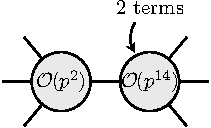
\includegraphics[trim={0cm 0cm 0cm 0cm},clip,scale=0.8]{14-fac-1}}+\raisebox{-5.5mm}{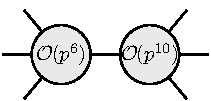
\includegraphics[trim={0cm 0cm 0cm 0cm},clip,scale=0.8]{14-fac-2}}\\
	&+\raisebox{-5.5mm}{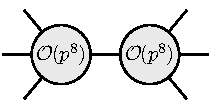
\includegraphics[trim={0cm 0cm 0cm 0cm},clip,scale=0.8]{14-fac-3}}+\raisebox{-6.5mm}{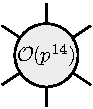
\includegraphics[trim={0cm 0cm 0cm 0cm},clip,scale=0.8]{14-contact}}.
\end{aligned}
$
\end{document}